\documentclass{article}

\usepackage{graphicx}
\usepackage{tikz}
\usepackage{tikzsymbols}
\usetikzlibrary{calc,patterns,shapes.geometric}
\pagestyle{empty}
\usepackage[margin=0pt]{geometry}
\geometry{papersize={14in,12in}}

\def\centerarc[#1](#2)(#3:#4:#5){\draw[#1] ($(#2)+({#5*cos(#3)},{#5*sin(#3)})$) arc (#3:#4:#5);}

\begin{document}
	\begin{figure}
		\centering
		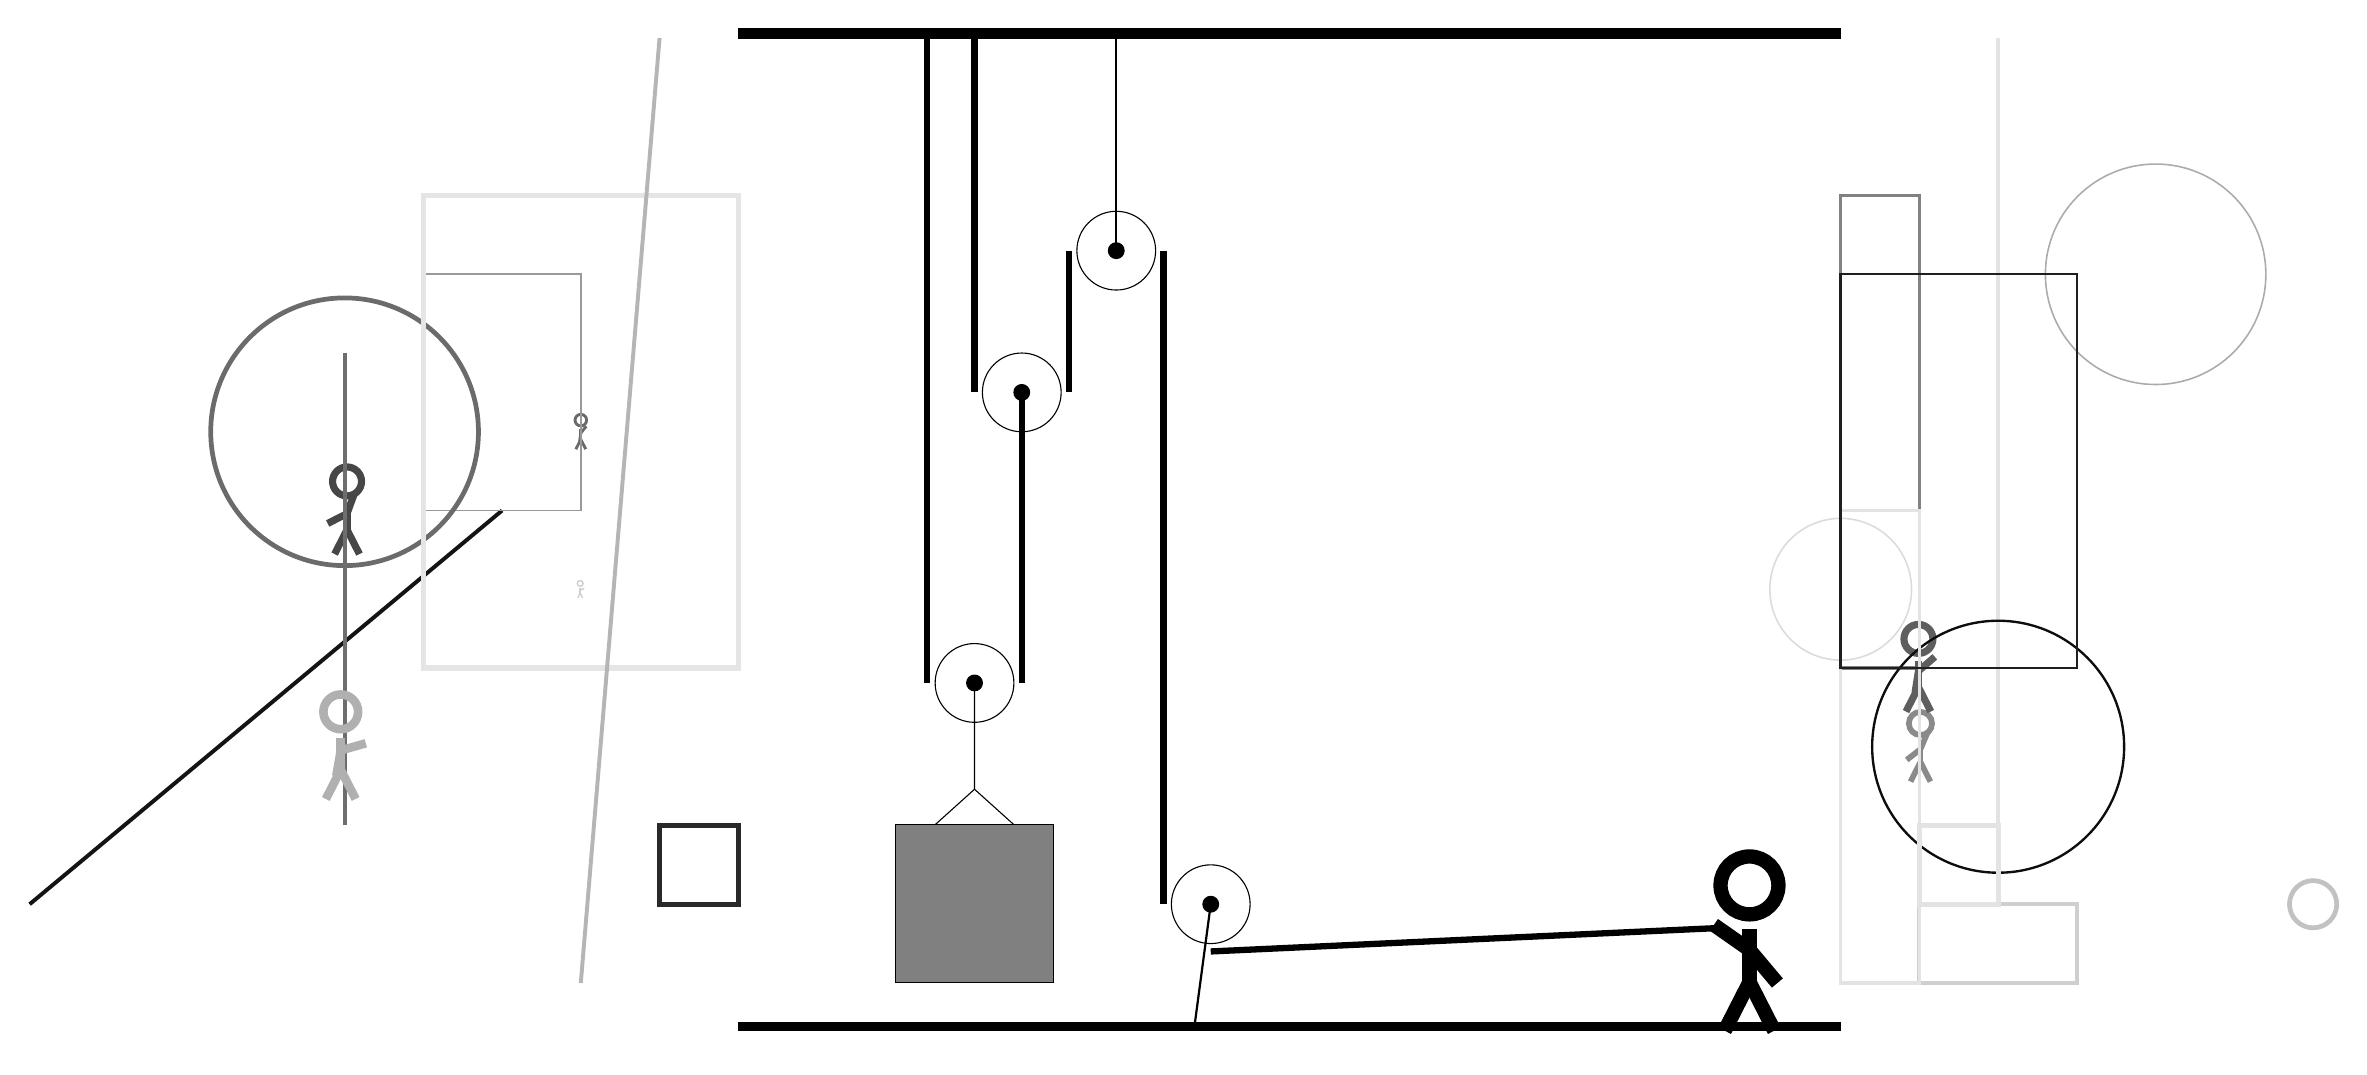
\begin{tikzpicture}
			%%%%% START %%%%%
			
			\draw[fill=black] (-2, 9) rectangle (12, 9.125);
			
			\draw (1, 0.81) circle (0.5);
			\draw[fill=black] (1, 0.81) circle (0.1);
			
			\draw (1.6, 4.5) circle (0.5);
			\draw[fill=black] (1.6, 4.5) circle (0.1);
			
			\draw (2.8, 6.3) circle (0.5);
			\draw[fill=black] (2.8, 6.3) circle (0.1);
			\draw[thick] (2.8, 6.3) -- (2.8, 9);
			
			\node[line width=0.6mm, color=black!59] at (-4, 4) {\Strichmaxerl[2][82][51]};
			
			\draw[line width=0.5mm, color=black!92](-5, 3) -- (-11, -2);
			\draw [line width=0.2mm, color=black!33](16, 6) circle (1.4);
			\draw[line width=0.5mm, color=black!19] (13, -3) rectangle (15, -2);
			\draw [line width=0.7mm, color=black!43](18, 5) circle (0.0);
			
			\draw [line width=0.2mm, color=black!14](12, 2) circle (0.9);
			
			\draw[line width=0.4mm, color=black!49] (12, 1) rectangle (13, 7);
			\node[line width=0.3mm, color=black!72] at (-7, 3) {\Strichmaxerl[5][27][70]};
			\draw[line width=0.6mm, color=black!84] (-2, -1) rectangle (-3, -2);
			\draw[line width=0.2mm, color=black!40] (-4, 3) rectangle (-6, 6);
			\node[line width=0.6mm, color=black!46] at (13, 0) {\Strichmaxerl[4][38][67]};
			
			\draw [line width=0.6mm, color=black!58](-7, 4) circle (1.7);
			\draw[line width=0.5mm, color=black!57](-7, -1) -- (-7, 5);
			
			\draw [line width=0.6mm, color=black!24](18, -2) circle (0.3);
			\draw[line width=0.5mm, color=black!19](14, 3) -- (14, 0);
			\draw[line width=0.5mm, color=black!11](14, 9) -- (14, -2);
			
			\node[line width=0.5mm, color=black!63] at (13, 1) {\Strichmaxerl[5][81][41]};
			
			\draw[line width=0.7mm, color=black!10] (-2, 7) rectangle (-6, 1);
			\draw [line width=0.3mm, color=black!95](14, 0) circle (1.6);
			\draw[line width=0.4mm, color=black!11] (12, -3) rectangle (13, 3);
			\draw[line width=0.5mm, color=black!29](-3, 9) -- (-4, -3);
			\node[line width=0.5mm, color=black!31] at (-7, 0) {\Strichmaxerl[6][80][16]};
			
			\draw[line width=0.6mm, color=black!11] (13, -1) rectangle (14, -2);
			\draw[line width=0.3mm, color=black!88] (12, 1) rectangle (15, 6);
			\node[line width=0.7mm, color=black!19] at (-4, 2) {\Strichmaxerl[1][90][17]};
			
			\draw (4.0, -2) circle (0.5);
			\draw[fill=black] (4.0, -2) circle (0.1);
			\draw[thick] (4.0, -2) -- (3.8, -3.5);
			
			\draw (1, 0.81) -- (1, -0.54) -- (0.5, -0.99) -- (1.5, -0.99) -- (1, -0.54);
			\draw[fill=black!50] (0, -0.99) rectangle (2, -2.99);
			\draw[line width=0.8mm] (0.4, 9) -- (0.4, 0.81);
			\centerarc[line width=0.8mm](1, 0.81)(180:360:0.6);
			\draw[line width=0.8mm](1.6, 0.81) -- (1.6, 4.5);
			\draw[line width=0.8mm] (1.0, 9) -- (1.0, 4.5);
			\centerarc[line width=0.8mm](1.6, 4.5)(180:360:0.6);
			\draw[line width=0.8mm](2.2, 4.5) -- (2.2, 6.3);
			\centerarc[line width=0.8mm](2.8, 6.3)(0:180:0.6);
			\draw[line width=0.8mm] (3.4, 6.3) -- (3.4, -2);
			\centerarc[line width=0.8mm](4.0, -2)(0:90:-0.6);
			\draw[line width=0.8mm](4.0, -2.6) -- (10.5, -2.3);
			
			\node at (10.8, -2.5) {\Strichmaxerl[10][-35][-50]};
			
			\draw[fill=black] (-2, -3.5) rectangle (12, -3.6);
			
			%%%%% END %%%%%
		\end{tikzpicture}
	\end{figure}	
\end{document}